\documentclass[border=10pt]{standalone}

\usepackage{tikz}
\usepackage{tikzsymbols}
\usetikzlibrary{calc,patterns,shapes.geometric}

\def\centerarc[#1](#2)(#3:#4:#5){\draw[#1] ($(#2)+({#5*cos(#3)},{#5*sin(#3)})$) arc (#3:#4:#5);}

\begin{document}
	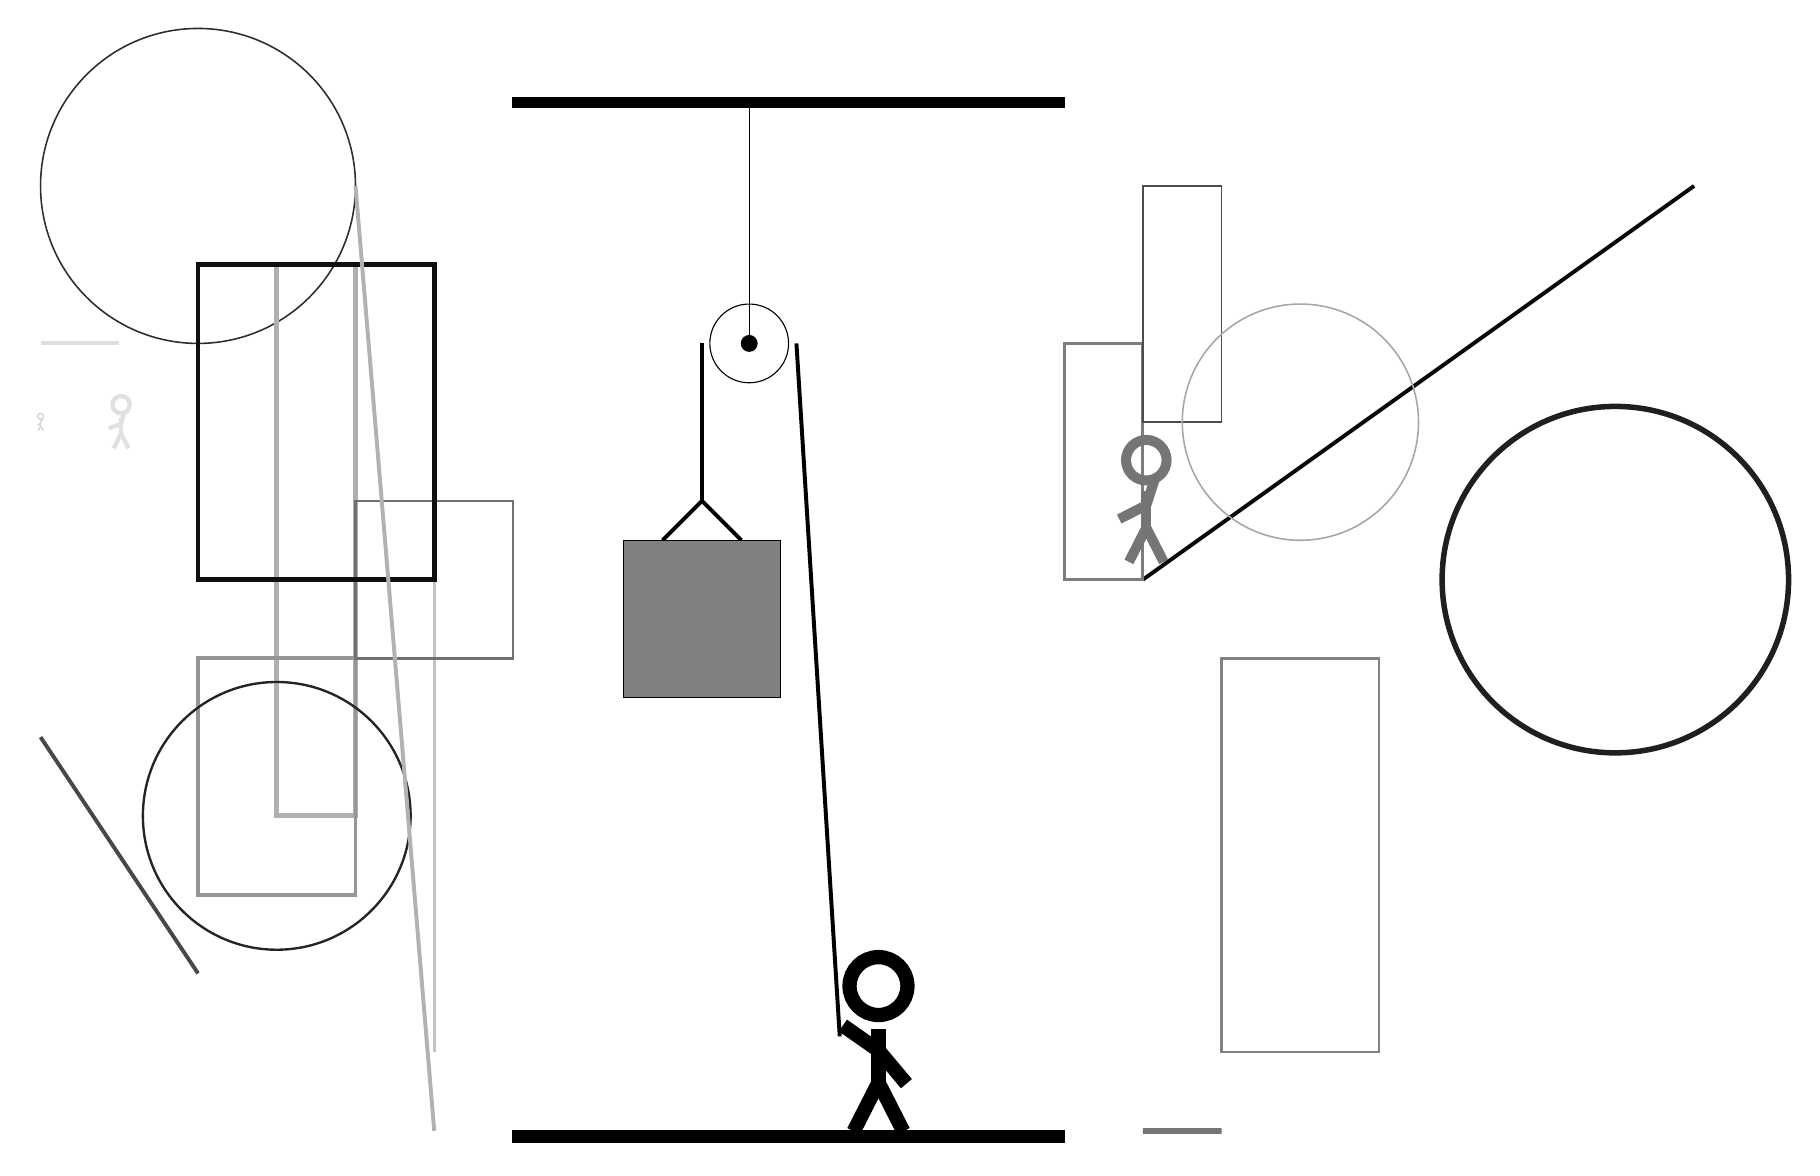
\begin{tikzpicture}
		%%%%% START %%%%%
		
		\draw[fill=black] (-2, 10) rectangle (5, 10.125);
		
		\draw[line width=0.5mm, color=black!97](6, 4) -- (13, 9);
		
		\draw [line width=0.2mm, color=black!82](-6, 9) circle (2.0);
		\draw[line width=0.7mm, color=black!54] (6, -3) rectangle (7, -3);
		\draw [line width=0.7mm, color=black!88](12, 4) circle (2.2);
		\draw[line width=0.3mm, color=black!49] (7, -2) rectangle (9, 3);
		\draw[line width=0.4mm, color=black!51] (5, 4) rectangle (6, 7);
		\draw[line width=0.4mm, color=black!23] (-3, 5) rectangle (-3, -2);
		\draw[line width=0.2mm, color=black!70] (7, 9) rectangle (6, 6);
		\node[line width=0.6mm, color=black!17] at (-8, 6) {\Strichmaxerl[1][47][61]};
		\draw[line width=0.6mm, color=black!31] (-4, 1) rectangle (-5, 8);
		\draw[line width=0.5mm, color=black!41] (-4, 3) rectangle (-6, 0);
		
		\draw [line width=0.3mm, color=black!86](-5, 1) circle (1.7);
		\node[line width=0.4mm, color=black!54] at (6, 5) {\Strichmaxerl[7][27][72]};
		
		\draw[line width=0.3mm, color=black!56] (-4, 3) rectangle (-2, 5);
		\draw[line width=0.5mm, color=black!12](-7, 7) -- (-8, 7);
		\draw[line width=0.5mm, color=black!72](-6, -1) -- (-8, 2);
		
		\draw [line width=0.2mm, color=black!35](8, 6) circle (1.5);
		\draw[line width=0.6mm, color=black!94] (-3, 4) rectangle (-6, 8);
		\draw[line width=0.5mm, color=black!30](-3, -3) -- (-4, 9);
		\node[line width=0.4mm, color=black!12] at (-7, 6) {\Strichmaxerl[3][19][77]};
		
		\draw (1, 7) circle (0.5);
		\draw[fill=black] (1, 7) circle (0.1);
		\draw (1, 10) -- (1, 7);
		
		\draw[line width=0.5mm] (-0.1, 4.5) -- (0.4, 5.0) -- (0.9, 4.5);
		\draw[fill=black!50] (-0.6, 4.5) rectangle (1.4, 2.5);
		
		\draw[line width=0.5mm] (0.4, 7) -- (0.4, 5.0);
		\centerarc[line width=0.5mm](1, 7)(0:180:0.6);
		\draw[line width=0.5mm](1.6, 7) -- (2.15, -1.8);
		
		\node at (2.6, -1.9) {\Strichmaxerl[10][-35][-50]};
		
		\draw[fill=black] (-2, -3) rectangle (5, -3.15);
		
		%%%%% END %%%%%
	\end{tikzpicture}
\end{document}